\documentclass{beamer}
\begin{document}
\subsection{Python -- Basic Syntax and Concepts}
    \begin{frame}[fragile]
        \frametitle{Python}
        \begin{itemize}
            \item A high-level, interpreted programming language
            \item Emphasizes readability and simplicity
            \item Widely used for web development, data analysis, artificial intelligence, and more
            \item Supported by a large community and a vast number of libraries
            \item Python is very intuitive to "read"; it uses mandatory indentation to visually signal the block structure of code: "Things that belong together are at the same indentation."
        \end{itemize}
    \end{frame}

    \begin{frame}{A Program and Programming}
        \begin{block}{What is a Program?}
            \textit{pro}- before + \textit{graphein} to write: to write in advance \\
            Computer scientist: a list of coded instructions for a computer
        \end{block}
        \begin{block}{What is Programming?}
            An act of writing a list of coded instructions for a computer
        \end{block}
    \end{frame}

    \begin{frame}[fragile]
        \frametitle{Introduction to Python}
        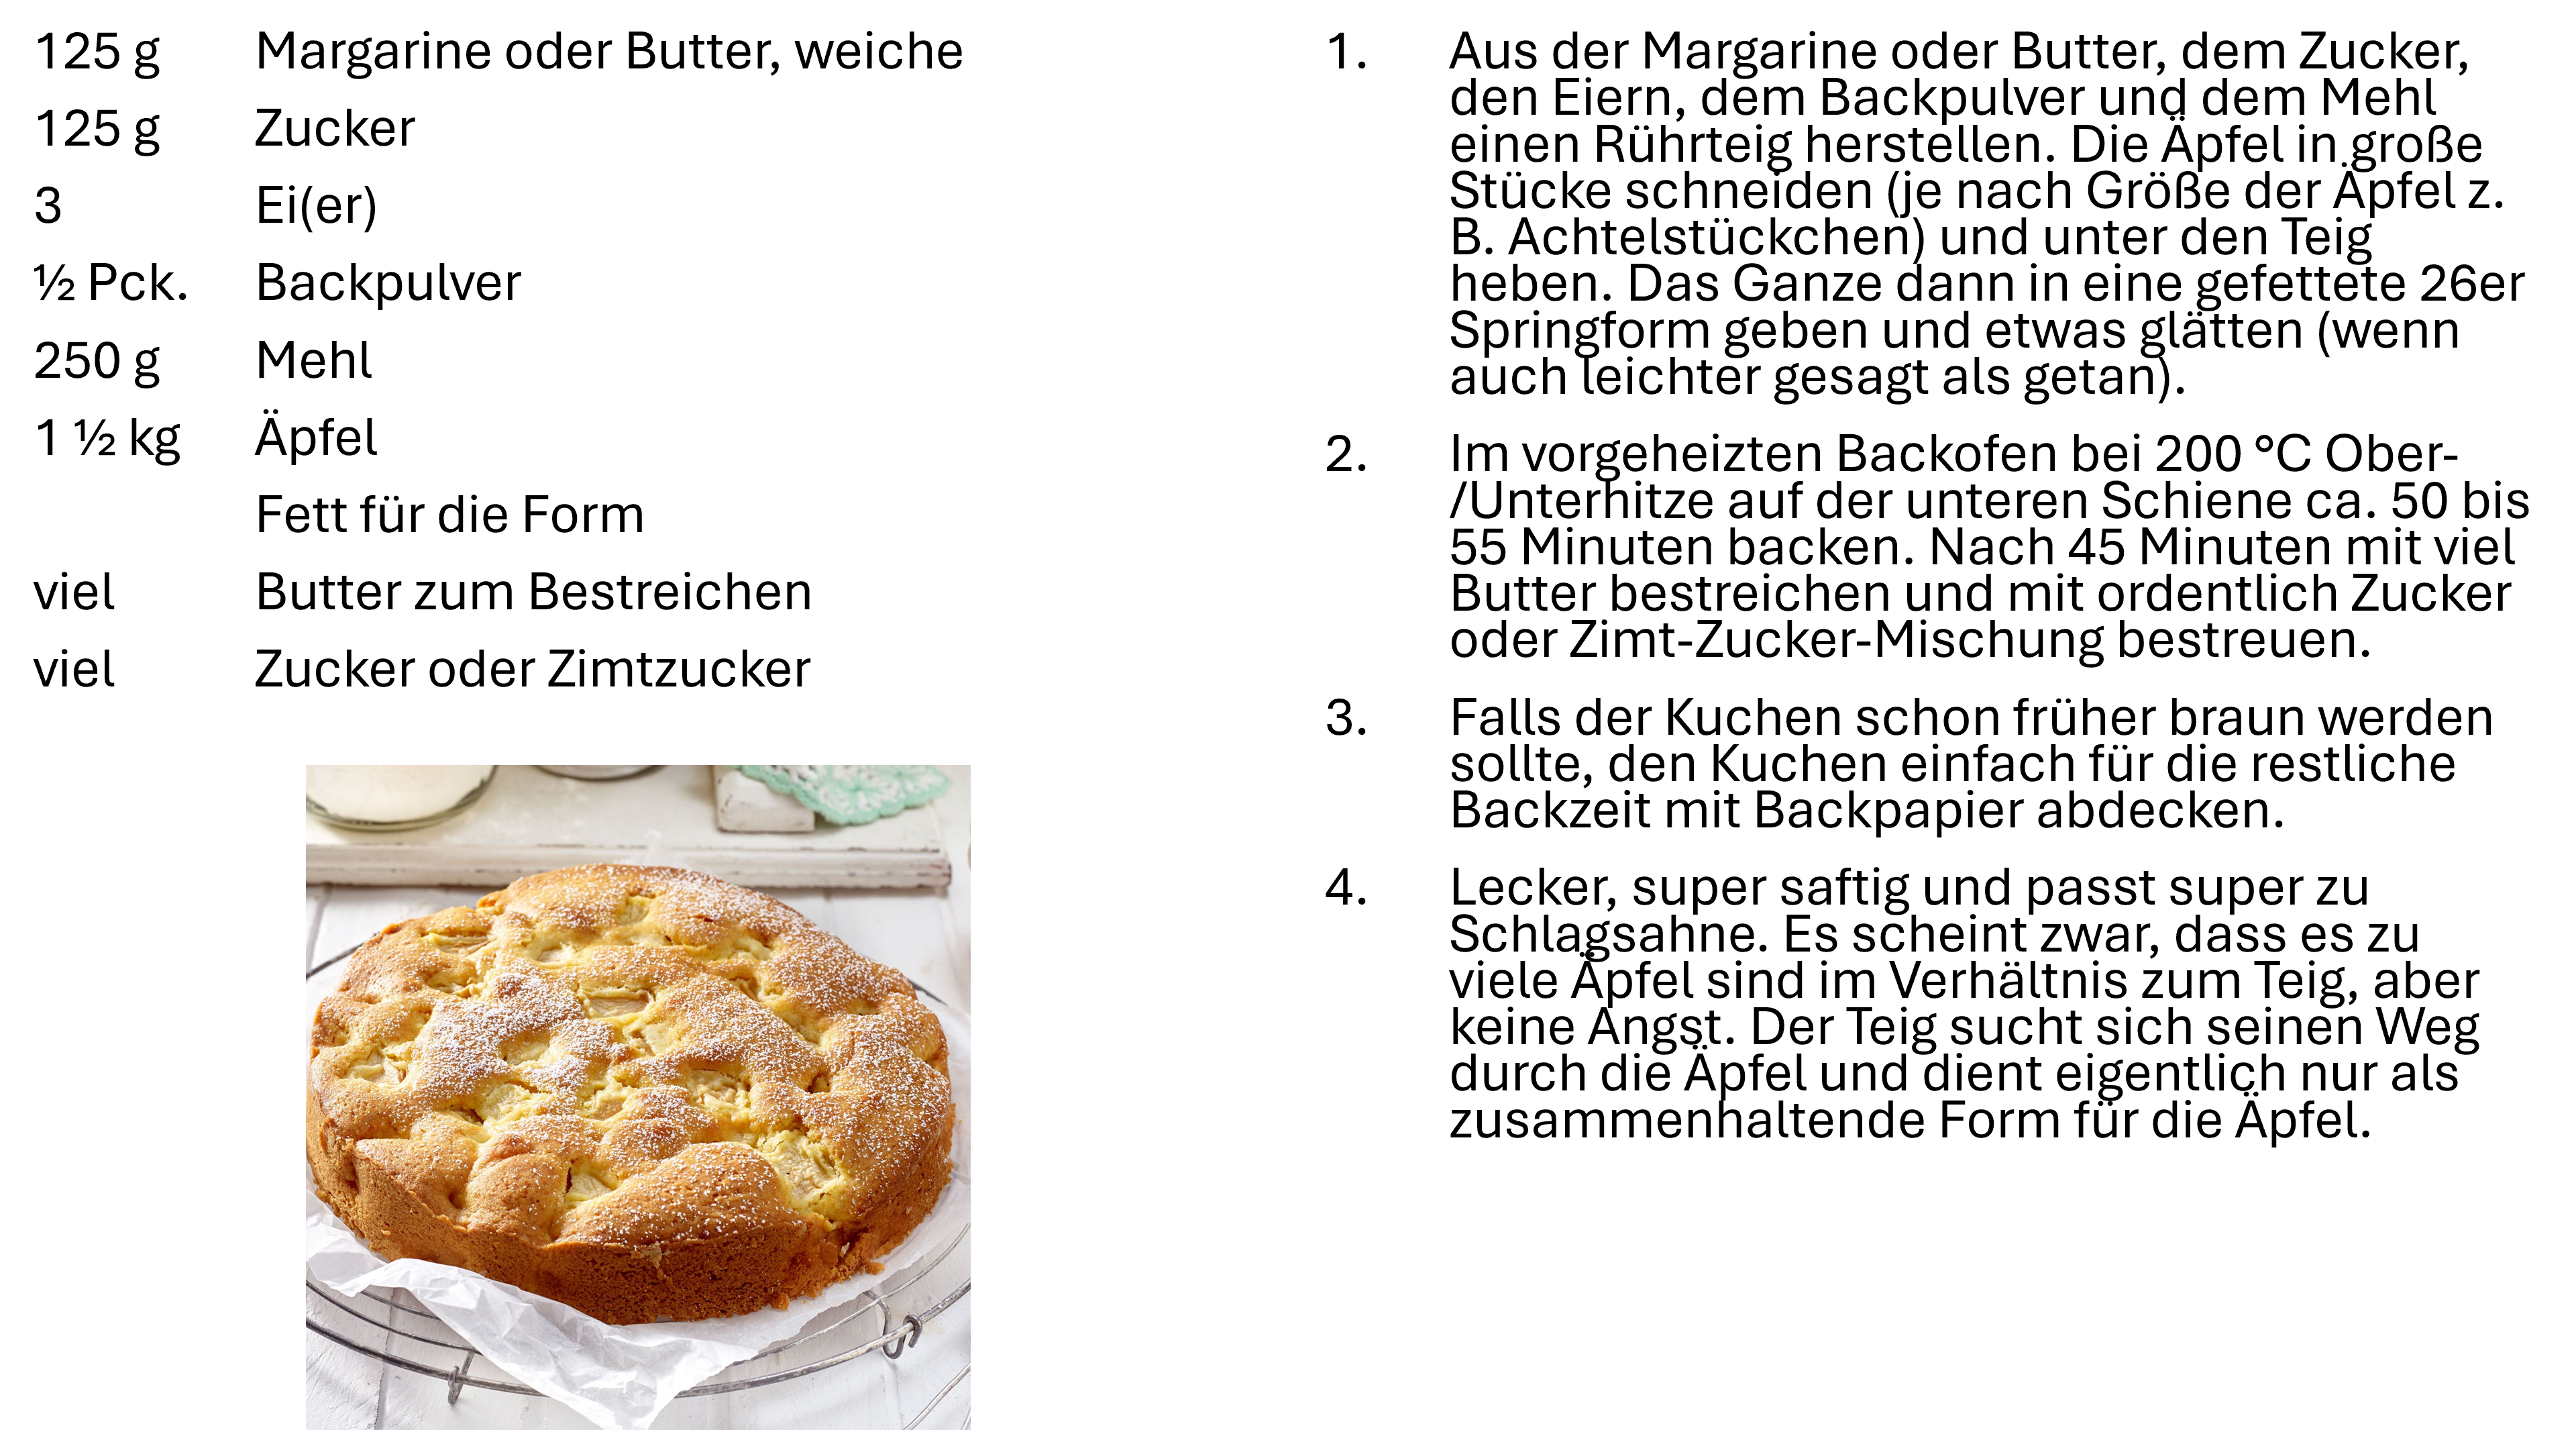
\includegraphics[width=1\textwidth]{figures/Recipe.png}
    \end{frame}

    % "fragile" and "lstlisting" envs are not compatible.
    \subsection{Ingredients of Python}
    \begin{frame}[fragile]
        \frametitle{Python Variables and Data Types}
        There are mainly five types of data within Python:
        \begin{itemize}
            \item Binary, e.g. Bytes
            \item Boolean, e.g. Truth value
            \item Numerical, e.g. Integer, Floating point
            \item String, e.g. Characters, Word
            \item Collection, e.g. List, Dictionary, Array
        \end{itemize}
    \end{frame}

    \begin{frame}[fragile]
        \frametitle{Python Binary and Boolean}
        Python's binary represents the low-level binary construct while the Boolean represents the truth value.
        \begin{itemize}
            \item Bytes
            \item Bytes Array
            \item Boolean (True, False)
        \end{itemize}
        \begin{exampleblock}{title}
            \begin{lstlisting}[language=python]
byte = b'\x01\x02\x03\x04\x05'
byte_array = bytearray(b'\x02\x03\x05\x07')
true = True
false = False
            \end{lstlisting}
        \end{exampleblock}
    \end{frame}

    \begin{frame}[fragile]
        \frametitle{Python Numerical}
        Python's numerical represents numbers.
        \begin{itemize}
            \item Integer
            \item Floating point
        \end{itemize}
    \end{frame}

    \begin{frame}[fragile]
        \frametitle{Python Integer}
        \begin{block}{Python Integer}
            \begin{itemize}
                \item Python integer represents the whole number in our understanding, stored in binaries.
                \item Typically has a fixed memory layout with different limitations.
            \end{itemize}
            \begin{center}
                \begin{tabular}{|c|c|}
                    \hline
                    \textbf{layout} & \textbf{range} \\
                    \hline
                    8-bit & -128 to 127 \\
                    16-bit & -32.768 to 32.767 \\
                    32-bit & -2.147.483.648 to 2.147.483.647 \\
                    64-bit & -9.223.372.036.... to 9.223.372.036.... \\
                    \hline
                \end{tabular}
            \end{center}
        \end{block}
        \begin{exampleblock}{8-bit Integer}
            \begin{center}
                \begin{tabular}{|c|c|c|c|c|c|c|c|}
                    \hline
                    0 & 1 & 0 & 0 & 0 & 1 & 0 & 1 \\
                    \hline
                \end{tabular}
            \end{center}
        \end{exampleblock}
    \end{frame}

    \begin{frame}[fragile]
        \frametitle{Python Floating Point}
        \begin{block}{Python Floating Point}
            \begin{itemize}
                \item Python floating point represents the decimal number in our understanding, stored in binaries.
                \item Typically has a fixed memory layout with different limitations.
                \item Unlike the integer, the floating point is an approximation of the real number.
            \end{itemize}
            \begin{center}
                \begin{tabular}{|c|c|}
                    \hline
                    \textbf{layout} & \textbf{range} \\
                    \hline
                    32-bit & -3.4E38 to 3.4E38 \\
                    64-bit & -1.7E308 to 1.7E308 \\
                    \hline
                \end{tabular}
            \end{center}
        \end{block}
    \end{frame}

    \begin{frame}[fragile]
        \frametitle{Python Floating Point}
        \begin{exampleblock}{Floating Precision}
            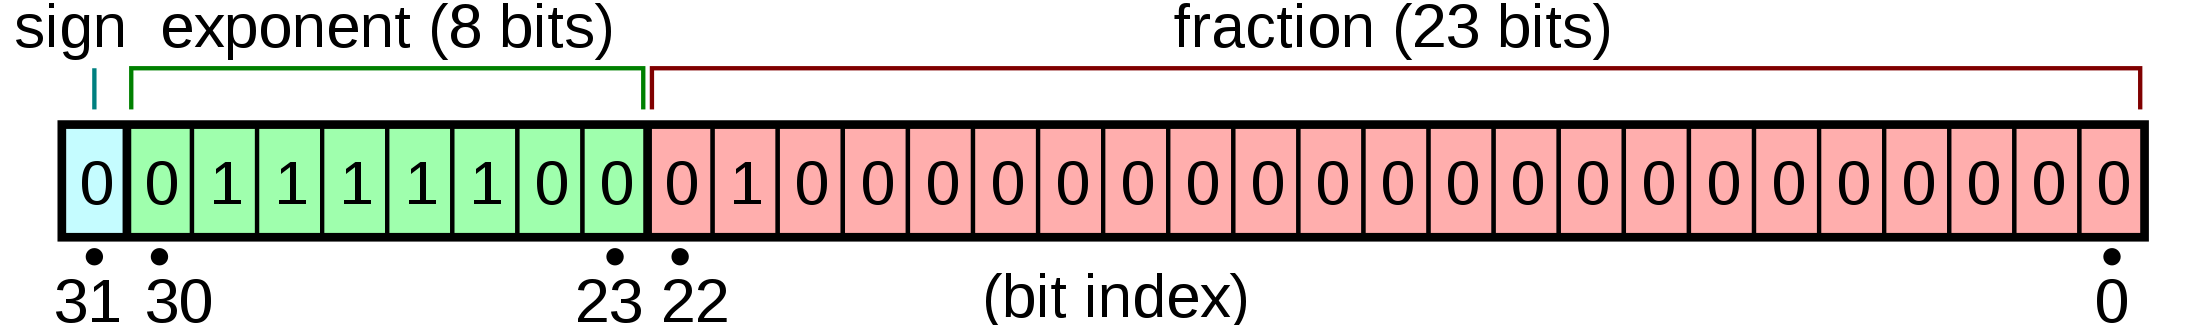
\includegraphics[width=1\textwidth]{figures/FP32.png}
            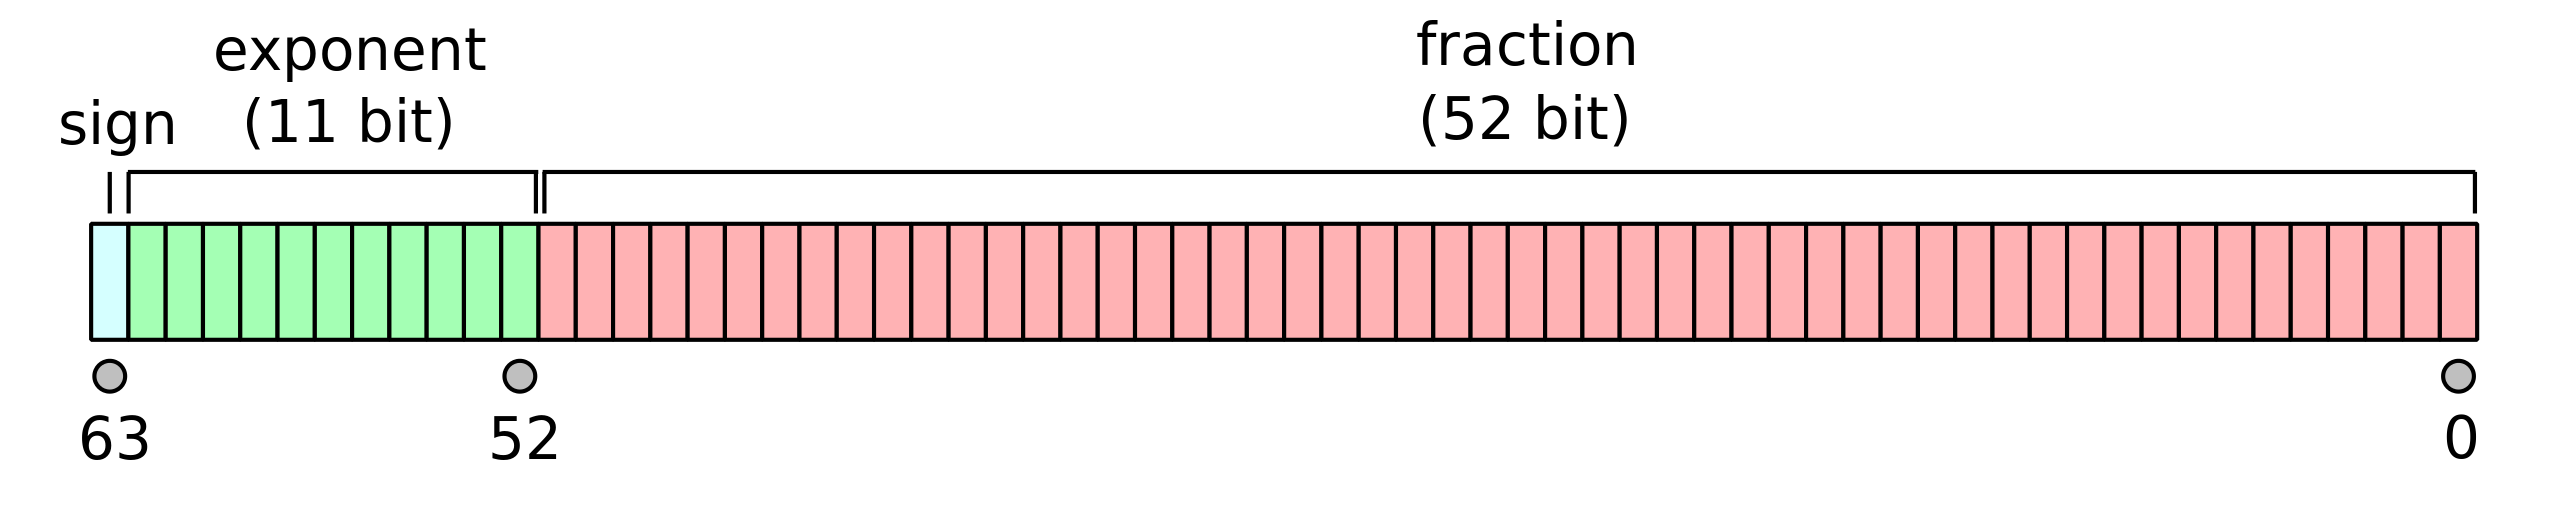
\includegraphics[width=1\textwidth]{figures/FP64.png}
        \end{exampleblock}
    \end{frame}

% \begin{frame}[fragile]
%     \frametitle{Python String}
%     \begin{itemize}
%         \item Python string is the character or word, stored in binaries.
%         \item Characters are stored as Unicode with an 8-bit memory layout.
%     \end{itemize}
% \end{frame}

    \begin{frame}[fragile]
        \frametitle{Python String}
        \begin{exampleblock}{ASCII table}
            \begin{center}
                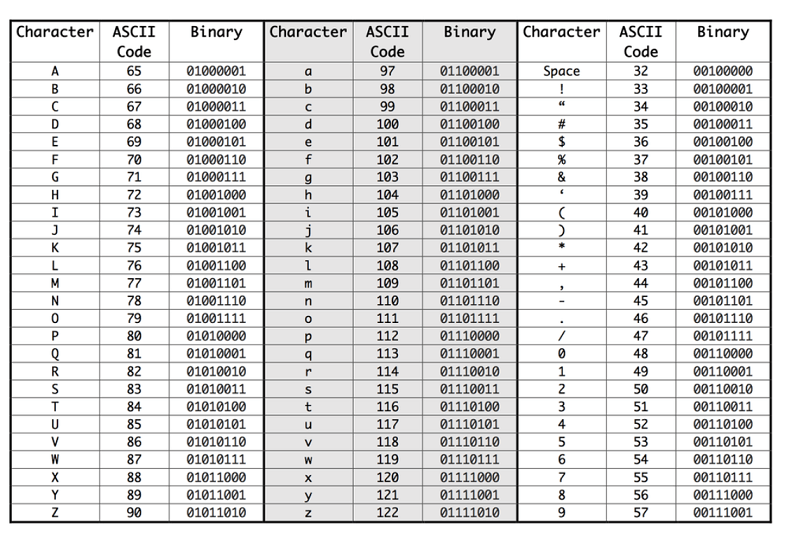
\includegraphics[width=0.8\textwidth]{figures/ascii-codes.png}
            \end{center}
        \end{exampleblock}
    \end{frame}

    \begin{frame}[fragile]
        \frametitle{Python Collections}
        \begin{itemize}
            \item Python collection is a collection of Python data and variables.
            \item All collections have a non-fixed memory layout.
            \item Common collections in Python:
            \begin{itemize}
                \item Sequences - List \& Tuple
                \item Mapping - Dictionary
            \end{itemize}
        \end{itemize}
    \end{frame}

    \begin{frame}[fragile]
        \frametitle{Python Sequences}
        \begin{itemize}
            \item Python sequences are versatile, ordered data structures
            \item Sequences can store elements of various data types, including numbers, strings, and other objects
            \item Sequences are useful when you do not know how many elements you want to include or if the number may change dynamically, e.g. a to-do list.
            \item Common sequences in Python:
        \end{itemize}
        \begin{exampleblock}{List \& Tuple}
            \begin{lstlisting}[language=Python]
List = [1, 2, 3, 4, 5]
Tuple = (1, 2, 3, 4, 5)
first_number = List[0]
            \end{lstlisting}
        \end{exampleblock}
    \end{frame}

    \begin{frame}[fragile]
        \frametitle{Python Mapping}
        \begin{itemize}
            \item Python mapping represents a collection of key-value pairs.
        \end{itemize}
        \begin{exampleblock}{Dictionary}
            \begin{lstlisting}[language=Python]
Dictionary = {'A': 1, 'B': 2, 'C': 3}
A = Dictionary['A']
            \end{lstlisting}
        \end{exampleblock}
    \end{frame}

    \begin{frame}[fragile]
        \frametitle{Defining Python Variables}
        To define a variable in Python, you simply assign a value to a name. As Python is dynamically typed, no need to specify the data type of the variable.
        \begin{block}{Syntax}
            \lstinline[language=python]{variable_name = value}
        \end{block}
        \begin{exampleblock}{Examples}
            \begin{lstlisting}[language=Python]
x = 42
fp = 3.14
string = "Hello, World!"
boolean = True
l = [1, 2, 3, 4, 5]
            \end{lstlisting}
        \end{exampleblock}
    \end{frame}

    \subsection{Instructions of Python}
    \begin{frame}[fragile]
        In the current era, there are 3 main schools of programming paradigms in Python:
        \begin{itemize}
            \item Imperative Programming
            \item Functional Programming
            \item Object-Oriented Programming
        \end{itemize}
    \end{frame}

    \begin{frame}[fragile]
        \frametitle{Programming Paradigm -- Procedural}
        Procedural programming is a programming paradigm where the program follows a procedural call pattern wherein contains a series of simple computational steps.
        \begin{example}
            \begin{lstlisting}[language=C++]
float twice(float x) { return x * 2.0; }
float half(float x) { return x / 2.0; }
int main() {
float a = 10.0;
float b = 20.0;

float c = twice(a);
float d = half(c+b);
return 0;
}
            \end{lstlisting}
        \end{example}
    \end{frame}

    \begin{frame}[fragile]
        \frametitle{Programming Paradigm -- Object-oriented}
        In object-oriented programming, the program is organized around objects, which are entities/Variables that contain data, in the form of fields/attributes; and code, in the form of procedures/methods.
        \begin{example}
            \begin{lstlisting}[language=Python]
class Calculator:
def __init__(self, a):
    self.a = a
def add(self, x):
    return self.a + x
cal = Calculator(10.0)
cal.add(20.0)
            \end{lstlisting}
        \end{example}
    \end{frame}

    \begin{frame}[fragile]
        \frametitle{Programming Paradigm -- Functional}
        Functional programming is a declarative programming paradigm consisting of a chain of functions. This paradigm uses a tree of expression that maps values to other values to construct a function.
        \begin{example}
            \begin{lstlisting}[language=Python]
session = DatabaseSession()
...
data = session.query(models.SensorData).filter(
models.SensorData.timestamp >= start_date_time,
models.SensorData.timestamp < end_date_time,
models.SensorData.sensor_id == sensor.sensor.id
).order_by(
models.SensorData.timestamp.asc()
).all()
            \end{lstlisting}
        \end{example}
    \end{frame}

    \subsection{Python Flow Control}
    \subsubsection{Conditional Statements: if, elif, and else}
    \begin{frame}[fragile]
        \frametitle{Conditional Statements: if, elif, and else}
        \begin{itemize}
            \item To execute conditional execution of code, we can use the If-control structure. Note the use of indentation to indicate what belongs together.
            \item Python supports \texttt{if}, \texttt{elif} (else if), and \texttt{else} for conditional statements
        \end{itemize}
        \begin{lstlisting}[language=Python]
x = 42

if x < 0:
    print("x is negative")
elif x == 0:
    print("x is zero")
else:
    print("x is positive")
        \end{lstlisting}
    \end{frame}

    \begin{frame}[fragile]{Flow Control}
        For mandatory alternative execution (where A or not A are executed), we can use the If-Else-control structure.
        \begin{lstlisting}[caption=Python Control Structures][language=Python]
# If-Else Statement

if x > 5:
print("x is greater than 5")
else:
print("x is not greater than 5")
        \end{lstlisting}
    \end{frame}

    \subsubsection{Loops: for and while}
    \begin{frame}[fragile]
        \frametitle{Loops: for}
        \begin{itemize}
            \item If the code needs to be repeated many times, we have loops.
            \item \texttt{for} loops are used to iterate over a sequence (such as a list or range or numbers) 
        \end{itemize}
        \begin{lstlisting}[language=Python]
print("Let's define a list of numbers")
numbers = [1, 2, 3, 4, 5]

print("Printing the variable num that, is assigned values from the list during the loop")
for num in numbers:
    print(num)
    print("In the loop")
print("Done.")
        \end{lstlisting}
    \end{frame}

    \begin{frame}[fragile]
        \frametitle{Loops: while}
        \begin{itemize}
            \item \texttt{while} loops are used to repeatedly execute a block of code as long as a condition is true. A list or range is not required; instead, we run it as long as the condition is true.
        \end{itemize}
        \begin{lstlisting}[language=Python]
print("Counting from 1 to 5")
count = 1

while count <= 5:
    print(count)
    print("Incrementing count")
    count += 1

print("Done counting.")
        \end{lstlisting}
    \end{frame}

    \subsubsection{Loop Control: break and continue}
    \begin{frame}[fragile]
        \frametitle{Loop Control: break}
        \begin{itemize}
            \item \texttt{break} is used to exit a loop prematurely
        \end{itemize}
        \begin{lstlisting}[language=Python]
for num in range(1, 10):
    print("Shall I break the loop?")
    if num == 5:
        print("Breaking the  loop")
        break
    print("Not yet broken the loop:")
    print(num)
print("Done.")
        \end{lstlisting}
    \end{frame}

    \begin{frame}[fragile]
        \frametitle{Loop Control: continue}
        \begin{itemize}
            \item \texttt{continue} is used to skip the current iteration (of a for loop) and proceed to the next one.
        \end{itemize}
        \begin{lstlisting}[language=Python]
for num in range(1, 10):
    print("Going to print num?")
    if num < 7:
        continue
    print(num)
print("Done.")
        \end{lstlisting}
    \end{frame}

    \subsection{Python Functions \& Methods}
    \begin{frame}[fragile]
        \frametitle{Python Functions}
        \begin{lstlisting}[caption=Python Functions][language=Python]
# Defining a function

def greet(name):
    return "Hello, " + name + "!"

# Calling a function

greeting = greet("Alice")
print(greeting)
        \end{lstlisting}
    \end{frame}

    \begin{frame}{Methods in Python}
        \begin{itemize}
            \item A method is a block of code that performs a specific task and is associated with an object or class.
            \item Methods are called using the dot notation, i.e. \texttt{object.method(arguments)}.
            \item Example: \\ \texttt{string="abc"} \\ \texttt{string.upper()}
        \begin{itemize}
            \item This method returns a copy of the string with all the letters converted to uppercase.
        \end{itemize}
        \end{itemize}
    \end{frame}
\end{document}